% \textbf{Title: Sampling 6}

Consider an analogue signal with this spectrum.

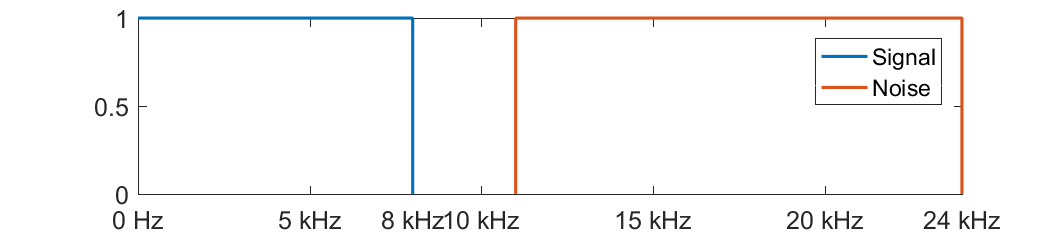
\includegraphics[width=6.27083in,height=1.375in]{../../Images/SamplingAndAliasingQ6.png}

Which of these sampling frequencies is the lowest we can use if we want to avoid aliasing between noise and the signal? The spectrum of the noise is an open interval. \\

a. \(21\ kHz\).

%@ Incorrect. This question tests the concept ``Sampling and Aliasing'', which is taught in these courses.

b. \(24\ kHz\).

%@ Incorrect. This question tests the concept ``Sampling and Aliasing'', which is taught in these courses.

*c. \(32\ kHz\).

%@ Correct! This question tests the concept ``Sampling and Aliasing'', which is taught in these courses.

d. \(48\ kHz\).

%@ Incorrect. This question tests the concept ``Sampling and Aliasing'', which is taught in these courses.

e. I do not know. \\

%@ It's okay. This question tests the concept ``Sampling and Aliasing'', which is taught in these courses.
